% =====================================================================
%  Appendix: complete flowcharts of the architecture
%  ---------------------------------------------------------------------
%  This is a fragment meant to be \input into the MDPI main document,
%  in the same way as the table fragments (e.g. tableA.tex). It assumes
%  \appendix has already been issued by the main document (the paper
%  already carries the appendix labelled app:protocol), so it does NOT
%  call \appendix itself. If this were the FIRST appendix, uncomment the
%  \appendix line below.
%
%  Graphics: the seven PNGs live in HIGH-LEVEL FLOWCHARTS/figures/.
%  Copy them into the paper's figures/ folder (the paper already resolves
%  images as figures/<name>), or add to the preamble:
%      \graphicspath{{figures/}{../HIGH-LEVEL FLOWCHARTS/figures/}}
%  Requires graphicx and the float package (H); both are provided by the
%  MDPI class used in the main document.
% =====================================================================

%\appendix   % uncomment only if this is the first appendix in the document

\section{Complete Flowcharts of the Architecture}
\label{app:flowcharts}

This appendix collects the complete flowcharts of the system behaviour outlined in Section~\ref{sec:methods}. Together they trace a device from power-on, through peer discovery, leader election and failover, to the answering of a user query. The diagrams share a common notation. Ovals are terminators (the entry and exit points of a flowchart); rectangles are processing steps; diamonds are decisions; and parallelograms are network input/output steps (a message sent to, or received from, another agent). Two conventions are specific to these diagrams. First, a coloured call box whose text reads "(see \dots\ diagram)" transfers control to the flowchart of the same colour: it is a jump to the referenced diagram rather than an ordinary step. Second, the green box with a dashed border denotes the leader's merged tool list, the shared data structure that stores the tools exposed by the sensing agents; steps that write it ("Merge into tool list", "Remove tool from tool list") or read it (the dashed "reads" arrow) operate on that structure. Each caption below is self-contained and can be read independently of the others.

\begin{figure}[H]
\centering
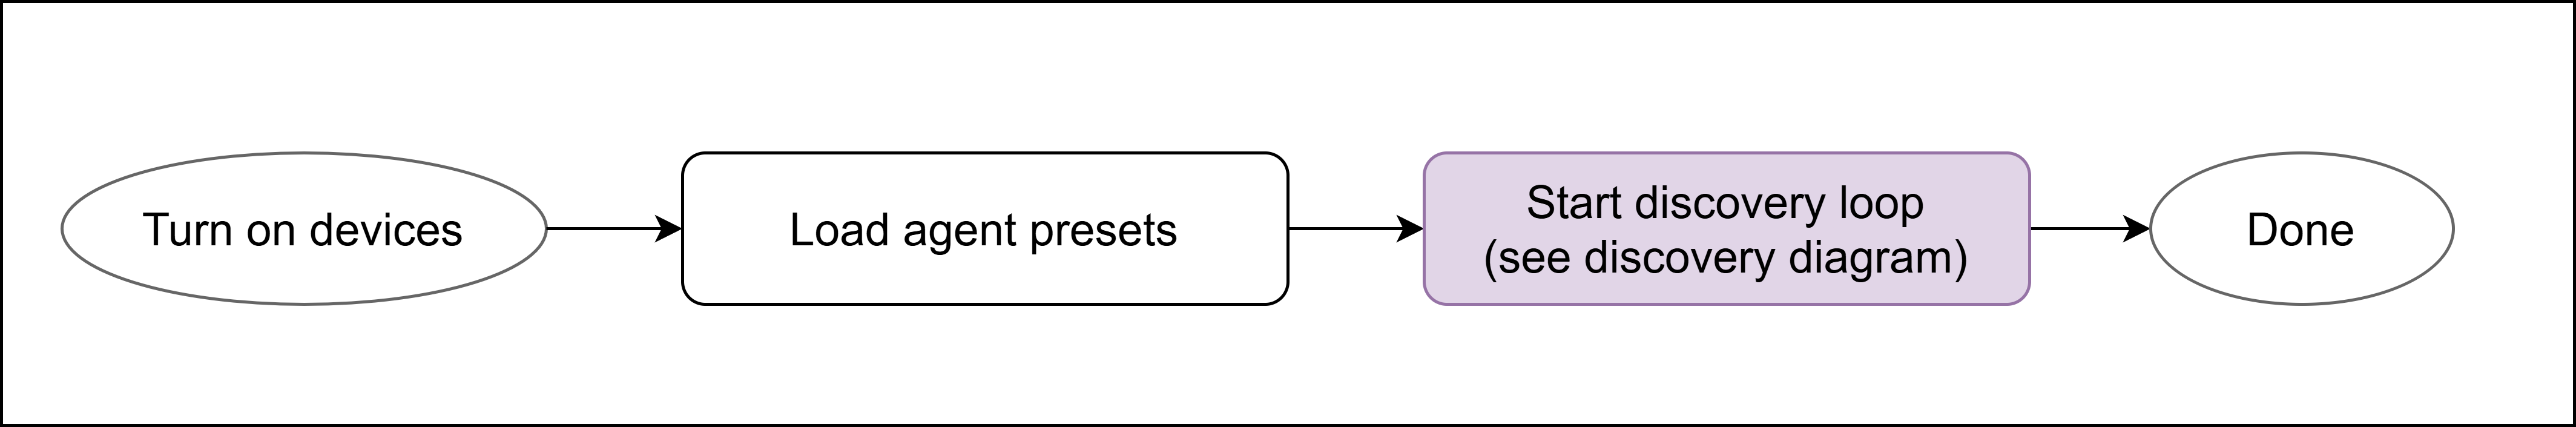
\includegraphics[width=\linewidth]{figures/1_startup.png}
\caption{Device startup sequence. When a device is powered on it first loads its agent presets from the local configuration (the presets decide which agents, sensing and/or leader, the device runs). It then enters the peer discovery loop, drawn as a coloured call box because control passes to the discovery flowchart of Figure~\ref{app:fig:discovery}. Discovery runs continuously for the lifetime of the device, so startup itself terminates once the loop has been launched.}
\label{app:fig:startup}
\end{figure}

\begin{figure}[H]
\centering
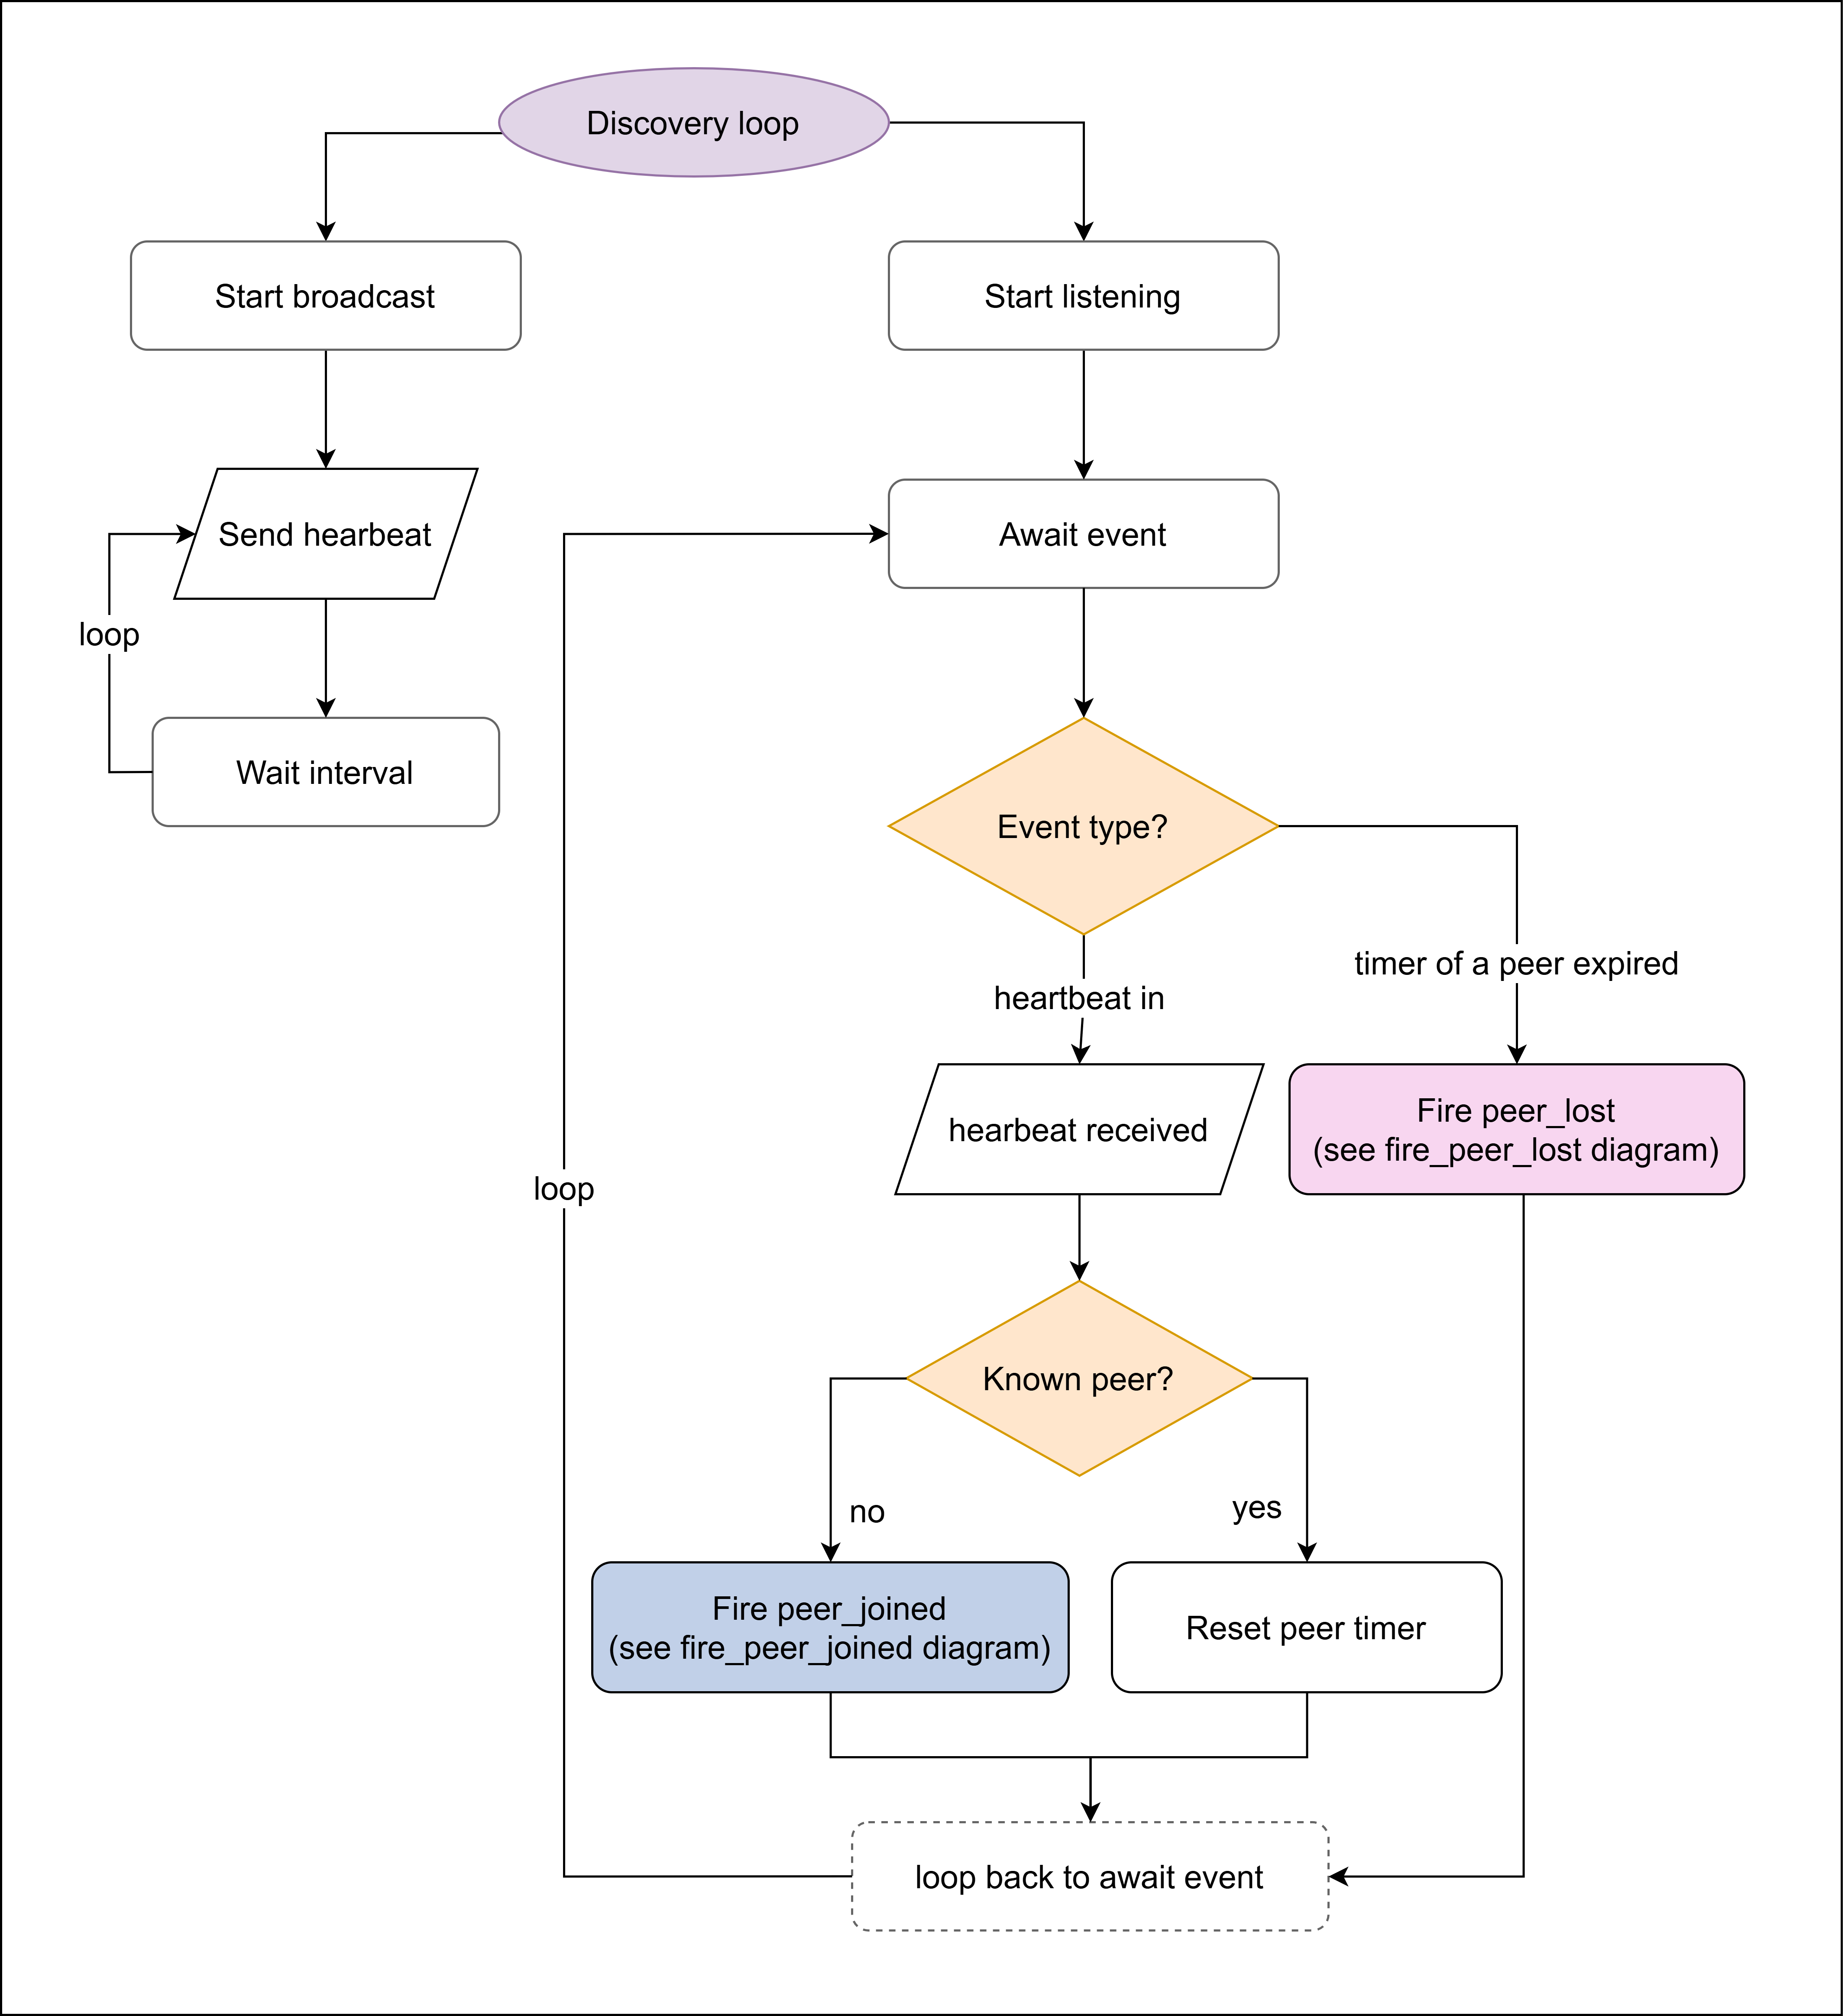
\includegraphics[width=\linewidth,height=0.92\textheight,keepaspectratio]{figures/2_discovery.png}
\caption{Peer discovery loop. The loop runs two concurrent activities. On the left, the device broadcasts: it periodically sends a heartbeat on the network and waits one interval before repeating, so that other devices learn it is alive. On the right, the device listens: it awaits an event and branches on the event type. A received heartbeat leads to a check on whether the sender is already a known peer; if it is not, the peer_joined handler is invoked (the coloured call box, detailed in Figure~\ref{app:fig:peerjoined}), otherwise the peer's liveness timer is reset. If instead a peer's timer expires (no heartbeat was received in time), the peer_lost handler is invoked (Figure~\ref{app:fig:peerlost}). After handling any event the device loops back to awaiting the next one.}
\label{app:fig:discovery}
\end{figure}

\begin{figure}[H]
\centering
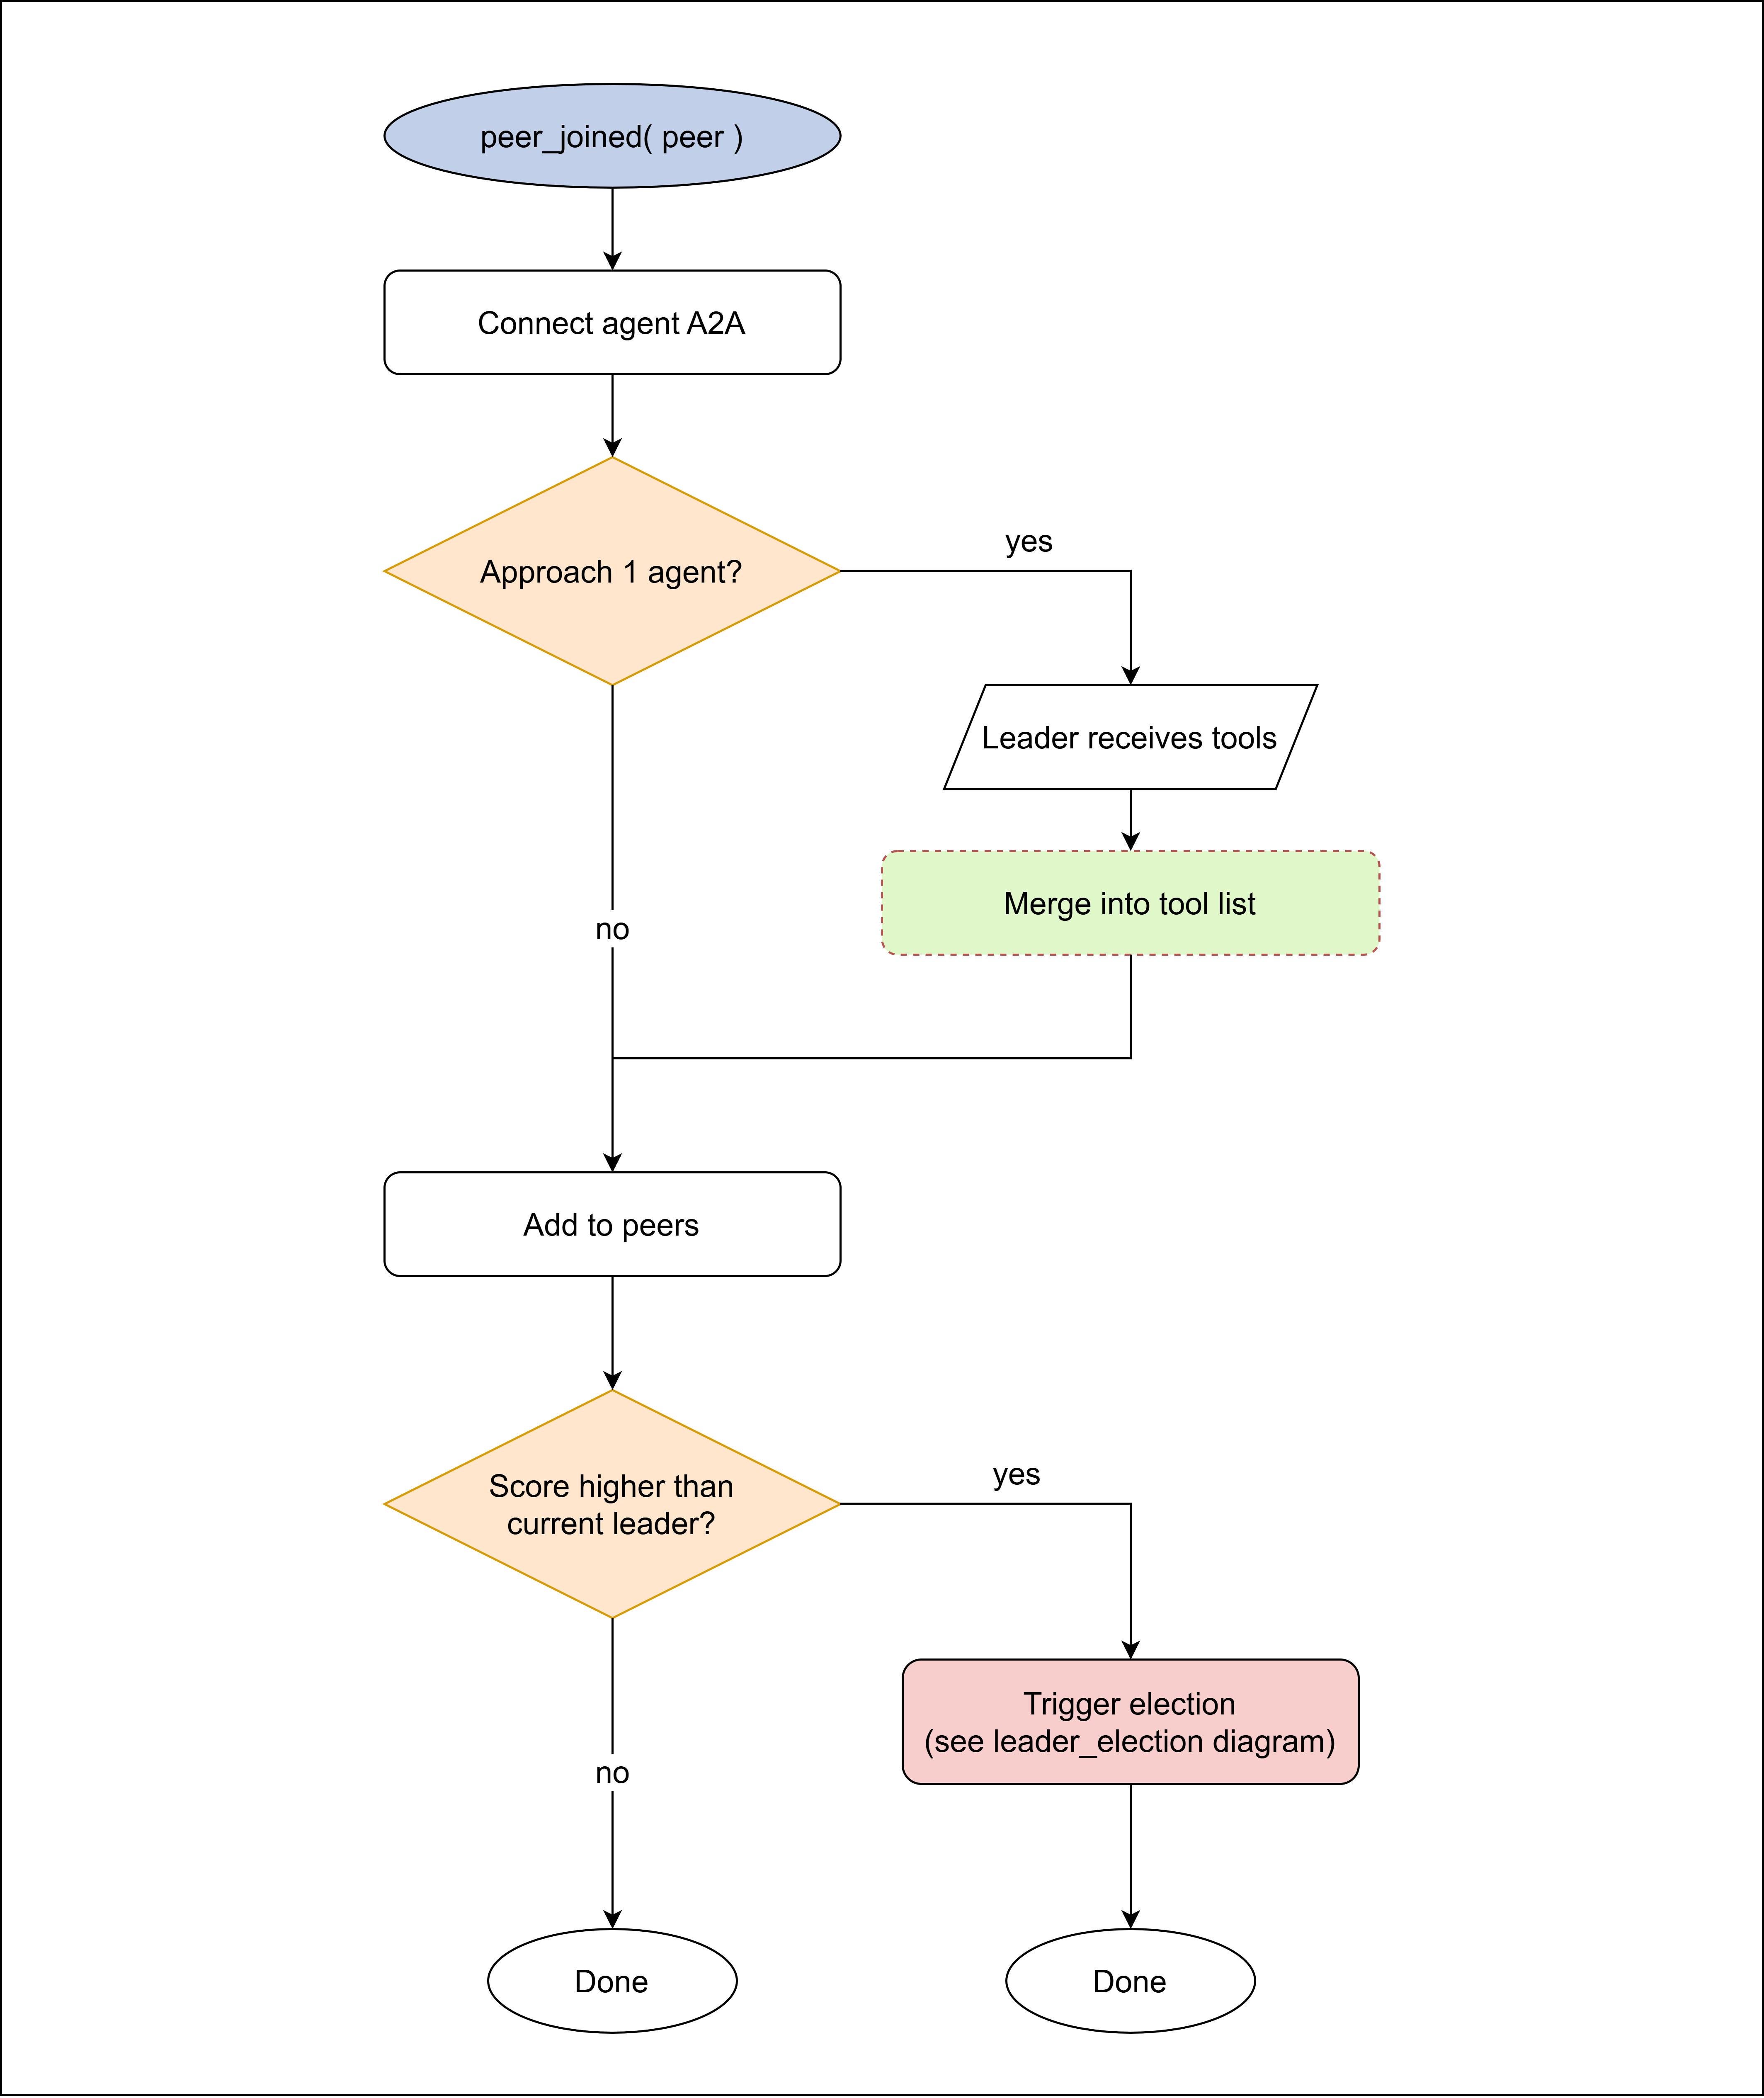
\includegraphics[width=\linewidth,height=0.92\textheight,keepaspectratio]{figures/3_peer_joined.png}
\caption{The peer_joined( peer ) handler, run when a previously unknown peer is discovered. The device first opens an agent-to-agent (A2A) connection to the new peer. If the peer is an Approach~1 sensing agent, the leader receives that peer's tool definitions and merges them into its tool list (removing duplicates); this branch is skipped for peers that do not expose tools this way. The peer is then added to the local peer set. Finally, if the new peer's device score is higher than that of the current leader, a leader election is triggered (the coloured call box, Figure~\ref{app:fig:election}) so that the more capable device can take over; otherwise the handler simply terminates.}
\label{app:fig:peerjoined}
\end{figure}

\begin{figure}[H]
\centering
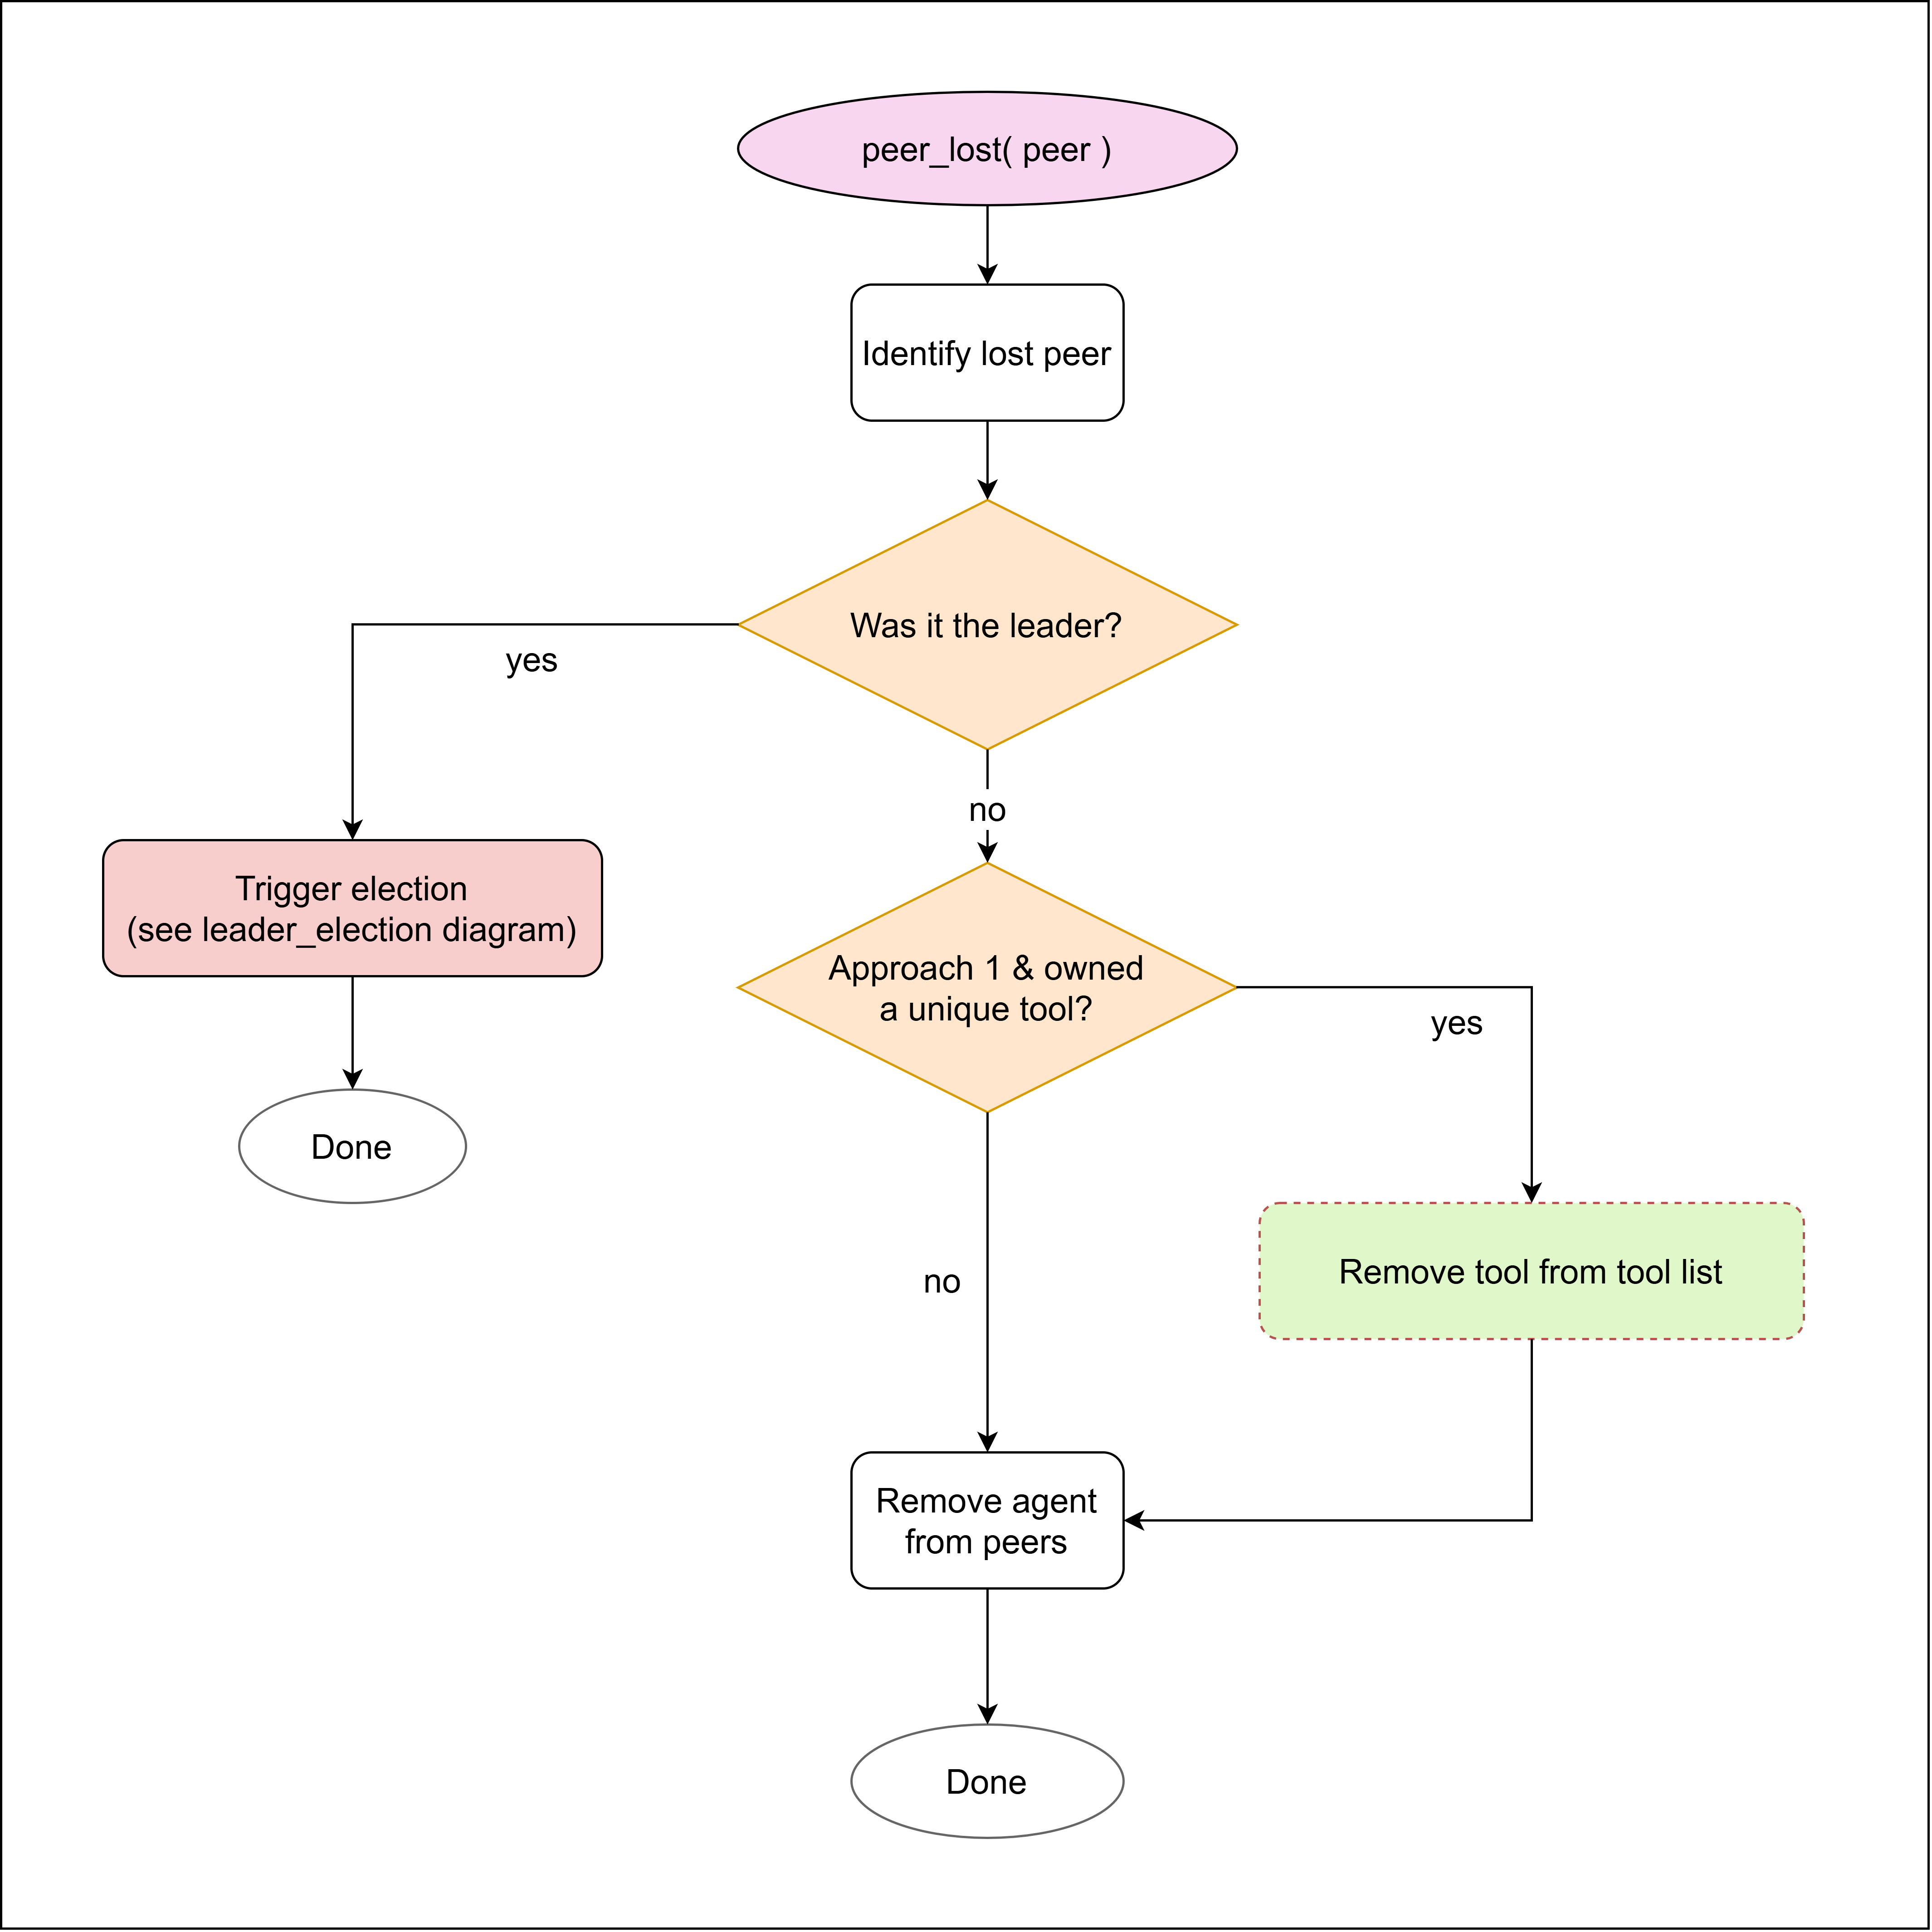
\includegraphics[width=\linewidth,height=0.92\textheight,keepaspectratio]{figures/4_peer_lost.png}
\caption{The peer_lost( peer ) handler, run when a peer's heartbeat times out. The device identifies the lost peer and checks whether it was the current leader. If it was, a leader election is triggered (the coloured call box, Figure~\ref{app:fig:election}) so that a surviving device can take over the coordinator role. If it was not the leader, the device checks whether the lost peer was an Approach~1 agent that owned a tool no other peer provides; in that case the tool is removed from the leader's tool list so that the LLM is no longer offered a tool that can no longer be executed. In all non-leader cases the peer is finally removed from the local peer set, and the handler terminates.}
\label{app:fig:peerlost}
\end{figure}

\begin{figure}[H]
\centering
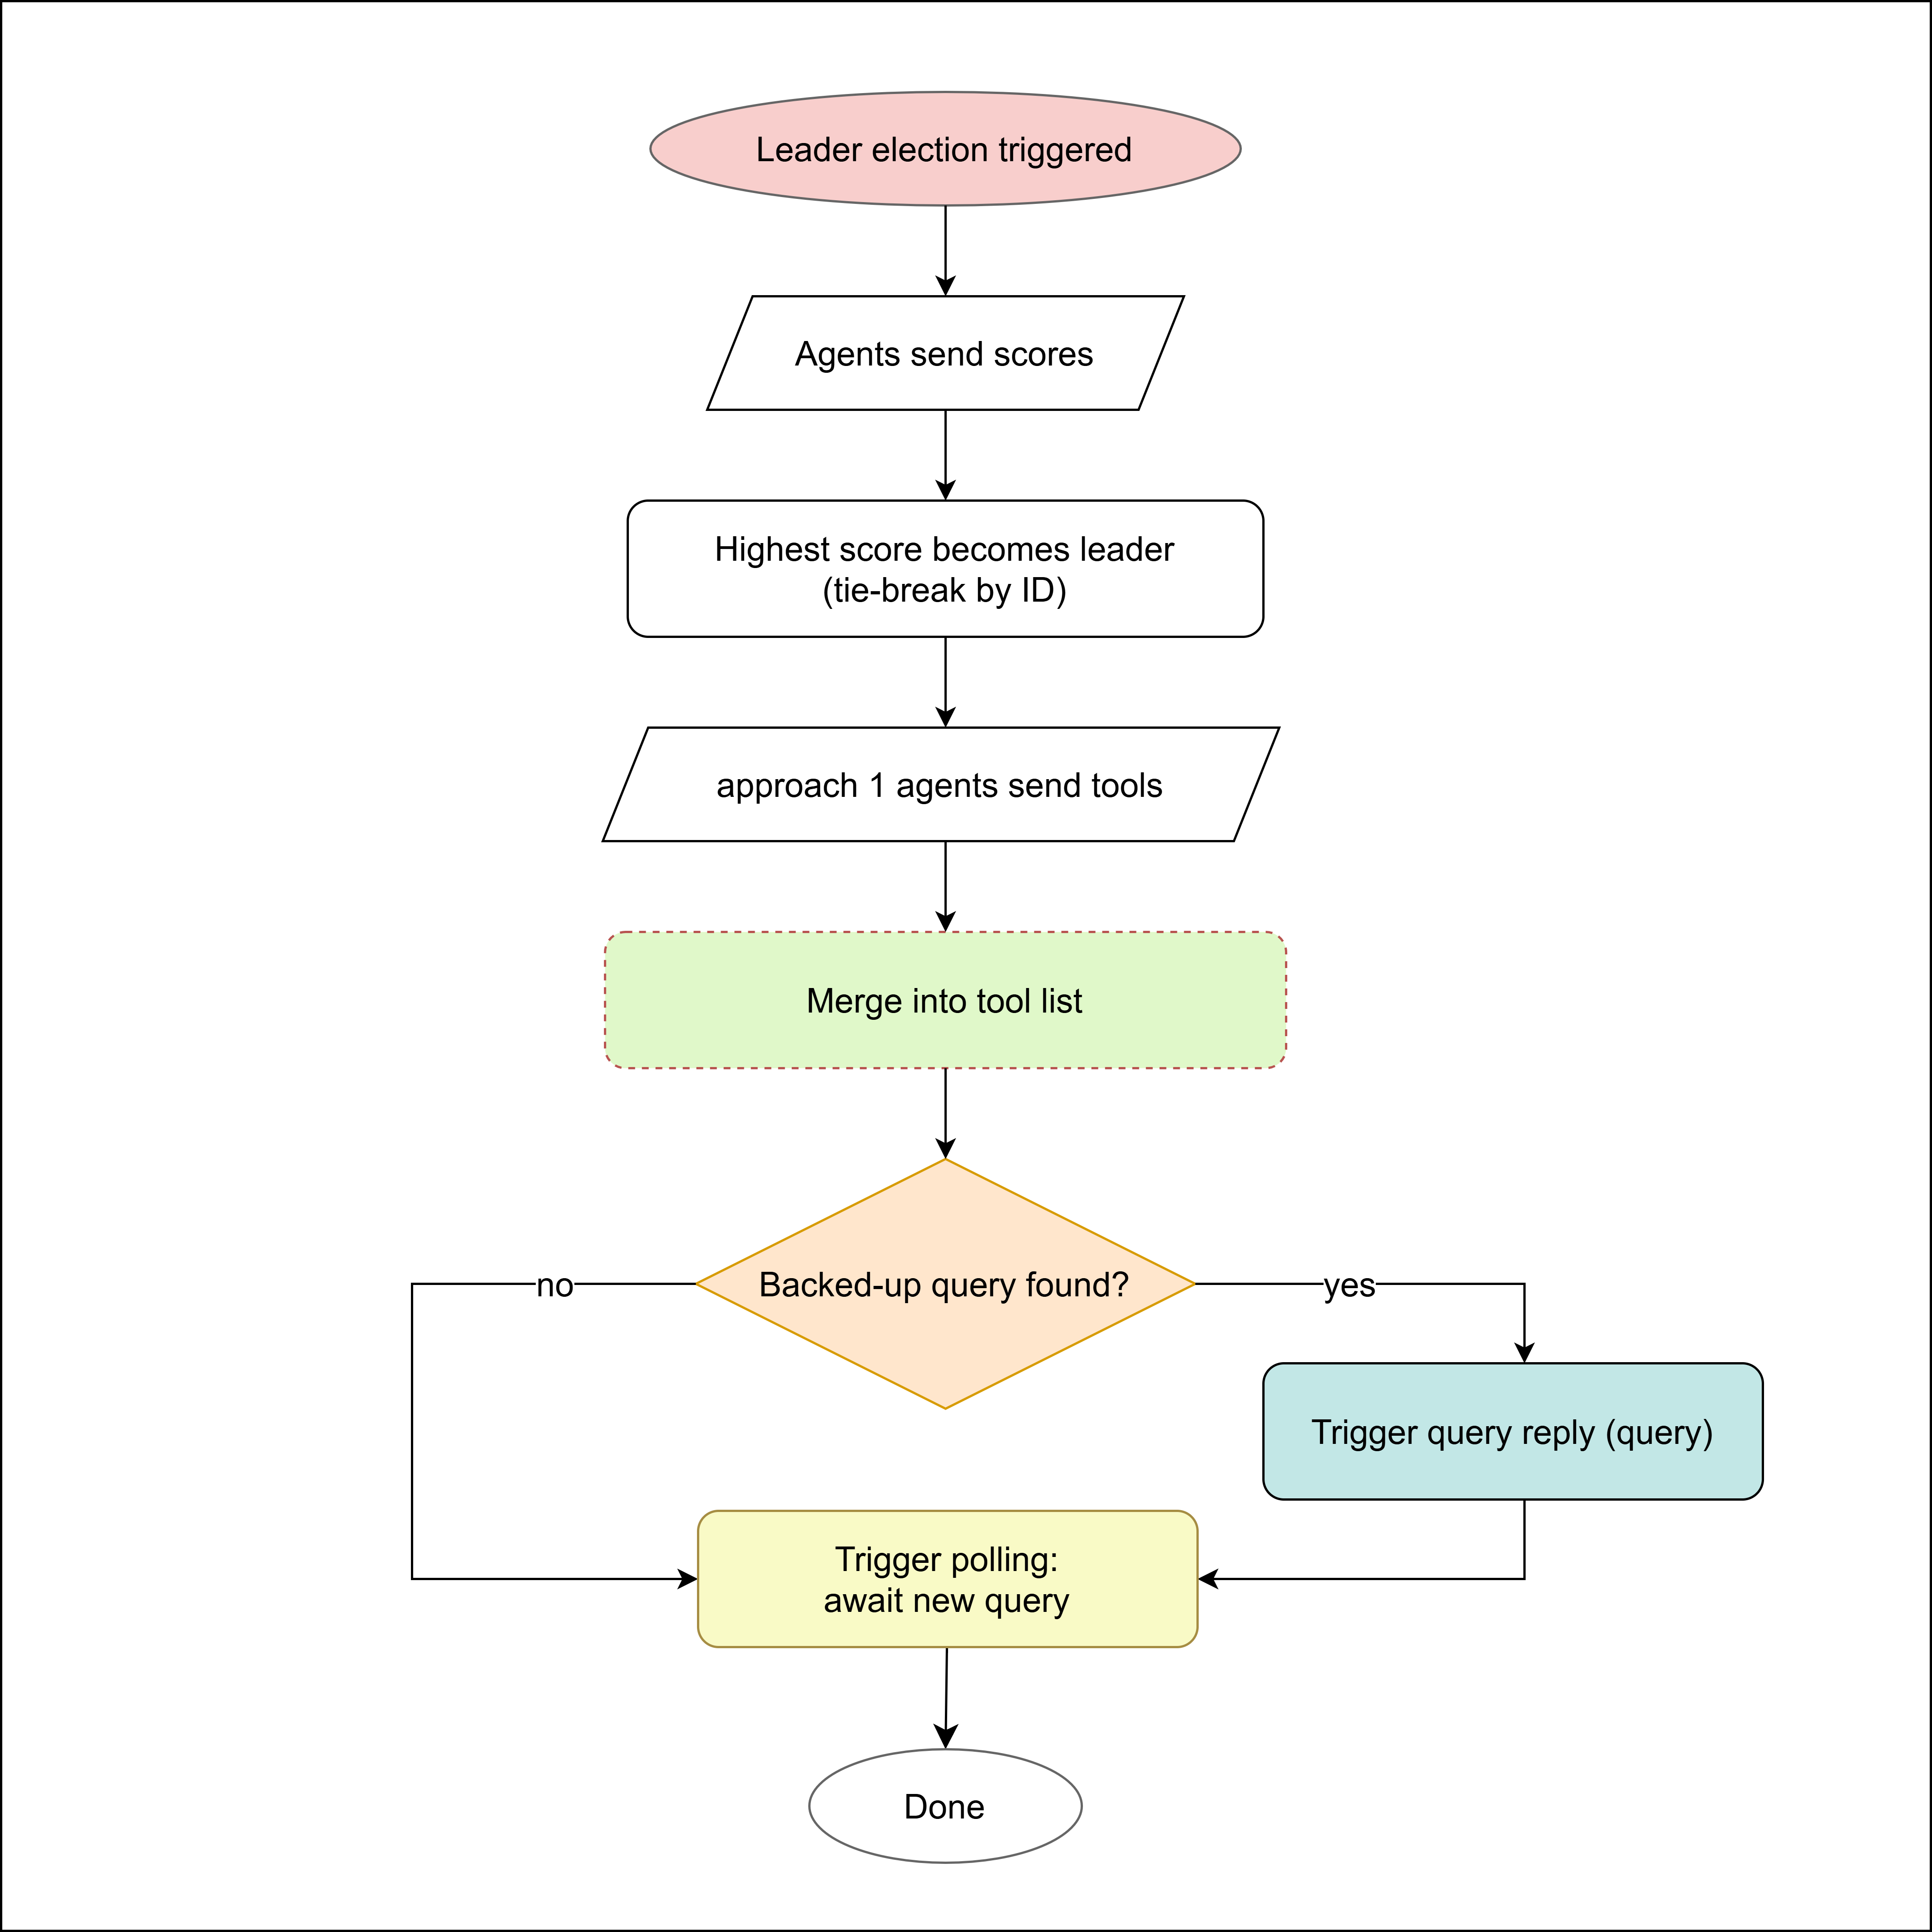
\includegraphics[width=\linewidth,height=0.92\textheight,keepaspectratio]{figures/5_leader_electionpng.png}
\caption{The leader election procedure, triggered when the leader is lost or when a more capable device joins. The candidate devices send their scores, and the device with the highest score becomes the new leader, with ties broken deterministically by agent-ID. The Approach~1 sensing agents then send their tools to the new leader, which merges them into its tool list. Because the previous leader may have been serving a request when it failed, the new leader checks whether a backed-up query was recovered from its replica: if so, it resumes that query by invoking the query reply procedure (the coloured call box, Figure~\ref{app:fig:queryreply}). Either way, the new leader ends by entering the polling loop that awaits the next user query (Figure~\ref{app:fig:polling}).}
\label{app:fig:election}
\end{figure}

\begin{figure}[H]
\centering
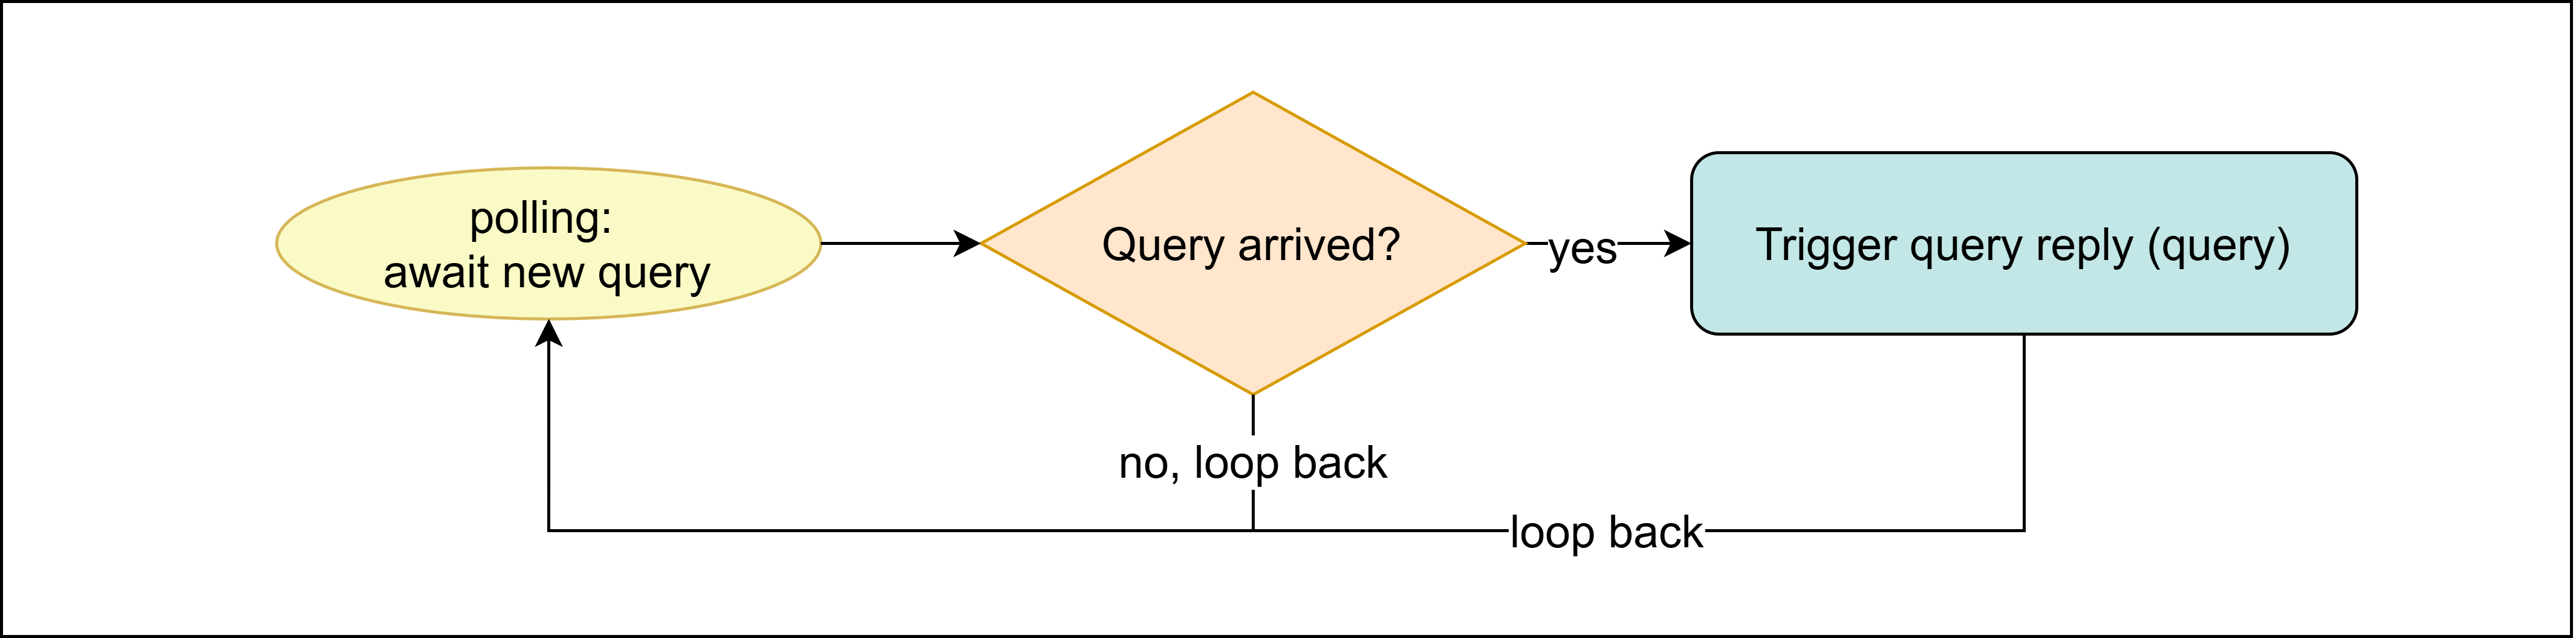
\includegraphics[width=\linewidth]{figures/6_polling_query.png}
\caption{The leader's polling loop for user queries. The leader waits for a new query and checks whether one has arrived. When a query arrives, it invokes the query reply procedure (the coloured call box, Figure~\ref{app:fig:queryreply}) to answer it and then loops back to await the next query; when no query has arrived, it simply loops back and keeps waiting. This loop is the leader's steady state between requests.}
\label{app:fig:polling}
\end{figure}

\begin{figure}[H]
\centering
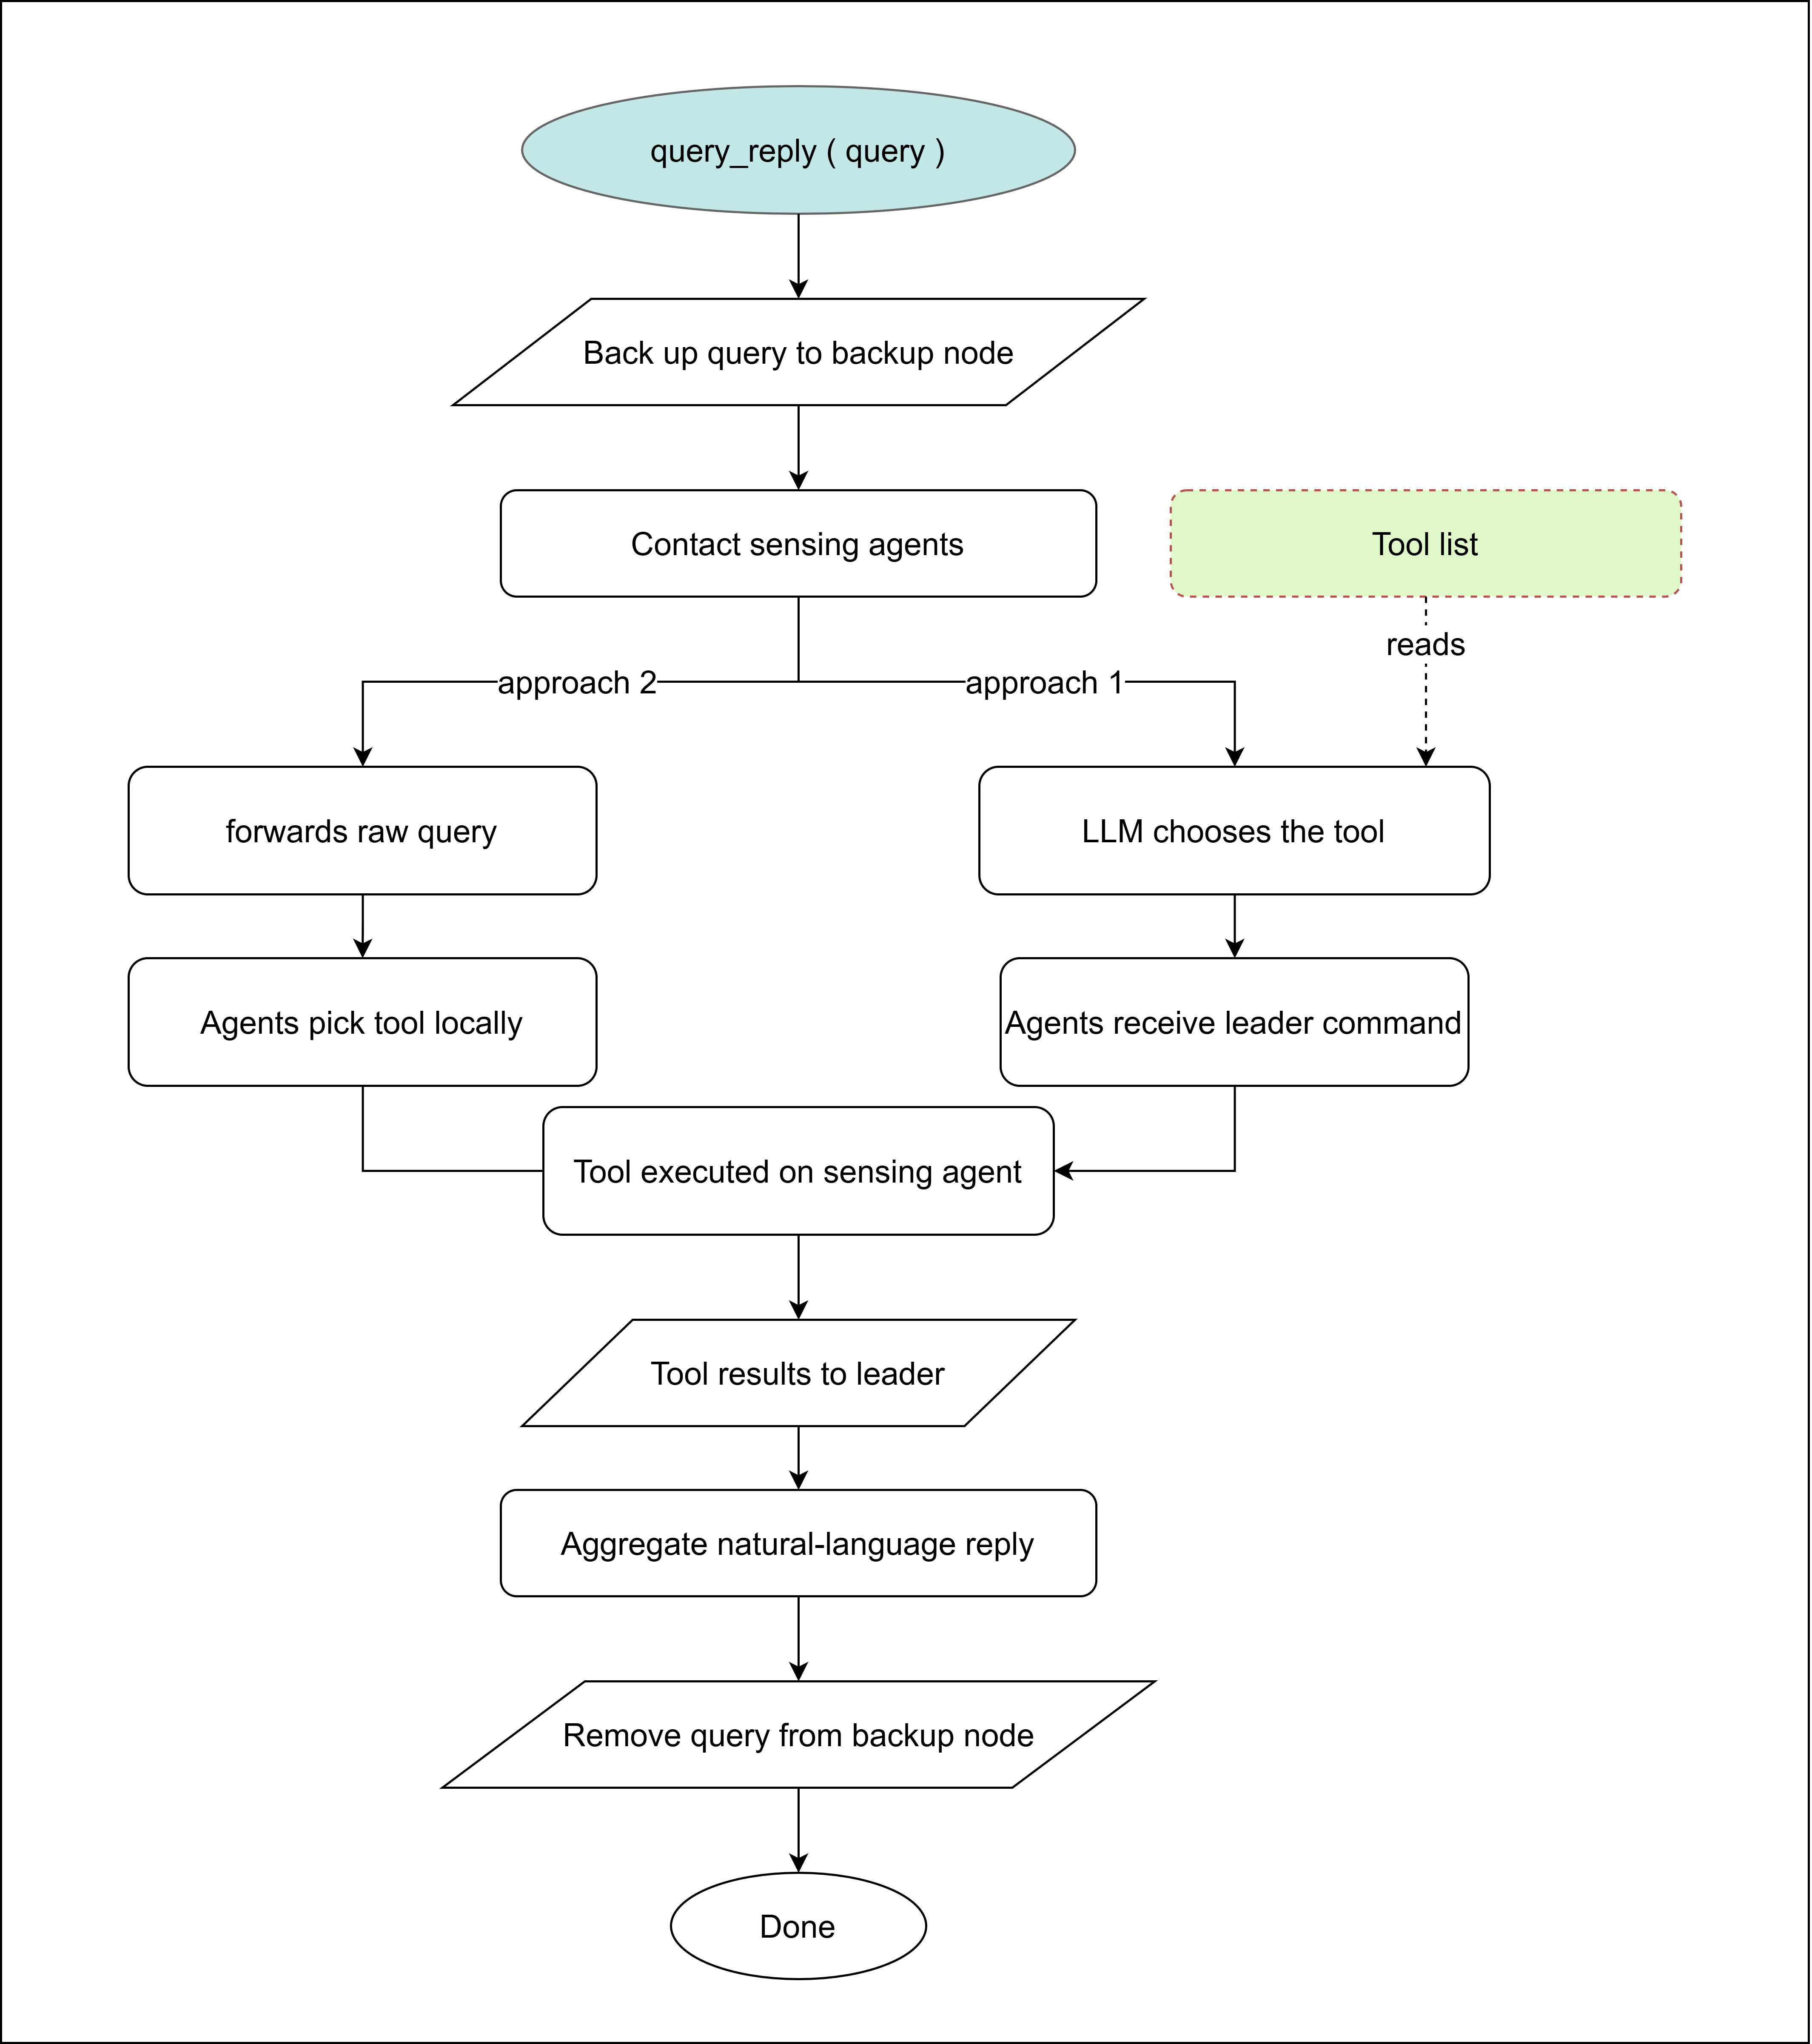
\includegraphics[width=\linewidth,height=0.92\textheight,keepaspectratio]{figures/7_query_reply.png}
\caption{The query_reply( query ) procedure that answers a single user query and is the point where the two approaches diverge. The leader first backs up the query to the backup node (the device with the second highest score) so that the request survives a leader failure, then contacts the sensing agents. Under Approach~2 the leader forwards the raw query and each sensing agent picks the matching tool locally. Under Approach~1 the leader's LLM chooses the tool, reading the candidate tools from the merged tool list (the dashed "reads" arrow), and the sensing agents receive the resulting command. In both cases the selected tool is executed on the sensing agent and its results are returned to the leader, which aggregates them into a single natural-language reply for the user. Finally the leader removes the now-served query from the backup node and the procedure terminates.}
\label{app:fig:queryreply}
\end{figure}

\FloatBarrier
